\documentclass[10pt,a4paper]{article}
\usepackage[margin=2cm]{geometry}
\usepackage{graphicx,booktabs,amsmath,hyperref,enumitem,listings,xcolor}
\usepackage[T1]{fontenc}
\lstset{basicstyle=\ttfamily\footnotesize,columns=fullflexible,frame=single,framerule=0.3pt,
        keywordstyle=\bfseries,language=C++,showstringspaces=false}
\setlist{nosep,leftmargin=1.5em}
\hypersetup{colorlinks,linkcolor=blue!50!black,urlcolor=blue!50!black}

\title{CS433 Assignment 2: Report\\\large Group \#1}
\author{Ashik Stenny \and Spandan Pati \and Vedhanth Balasubramanian}
\date{October 2026}

\begin{document}
\maketitle

\section*{Files and build}
We submit two source files. Each one builds several programs, selected with a compile-time flag:
\begin{itemize}
\item \texttt{q1\_mpsc.cpp} (Question 1), versions P1--P4:\\
      \texttt{g++ -O2 -DVERSION=k -o q1\_pk q1\_mpsc.cpp -lpthread} \quad ($k = 1..4$)\\
      Usage: \texttt{./q1\_pk N P n}. The consumed values go to standard output; a summary line with the time goes to standard error.
\item \texttt{q2\_graph.cpp} (Question 2), versions P1--P6:\\
      \texttt{g++ -O2 -DVERSION=k -o q2\_pk q2\_graph.cpp -lpthread} \quad ($k = 1..6$)\\
      Usage: \texttt{./q2\_pk op\_file op\_count num\_threads}, which reads the first \texttt{op\_count} lines of \texttt{op\_file}.\\
      The operation-file generator is in the same file:\\
      \texttt{g++ -O2 -DGEN\_OPS -o gen\_graph\_ops q2\_graph.cpp -lpthread}\\
      Usage: \texttt{./gen\_graph\_ops op\_count ins\% del\% num\_vertices out\_file [seed]}, e.g.\ \texttt{./gen\_graph\_ops 4000000 30 30 10000 ops.txt}.
\end{itemize}
The FIFO/fairness test program and the benchmark and plotting scripts that we used for the experiments are not part of the submission.
Only POSIX threads and standard C/C++ are used. Every program checks its own output after the timed region
(Q1: every value consumed exactly once and in per-producer order; Q2: every list strictly sorted and
the final edge count equal to initial edges + successful inserts $-$ successful deletes). All runs reported below passed these checks.

\paragraph{Platform.} AMD Ryzen 7 5800HS (8 cores, 16 hardware threads, one socket, 16\,MB L3), Linux 6.17, g++ 15.2, \texttt{-O2}.
Each configuration was run 3 times and the median is reported. Time is measured with \texttt{gettimeofday} around thread creation,
the parallel work and the joins only. Allocating and initialising data structures, reading the op file, building the initial graph,
printing and checking are all outside the timed region.

%=====================================================================
\section{Question 1: lock-free FIFO semaphore and multi-producer single-consumer}

\subsection{The lock-free semaphore (P1)}
The only atomic primitive is the class's \texttt{CompareAndSet} (\texttt{lock cmpxchgl}). From it we build a lock-free
\texttt{FetchAndInc}: read the value, CAS it to value$+1$, retry if the CAS fails. A failed CAS means another
thread's CAS succeeded, so the system as a whole always makes progress (lock-free). No lock is built from the CAS.

The semaphore is a \emph{ticket semaphore} with two counters:
\begin{itemize}
\item \texttt{ticket}: the number of \texttt{wait} calls that have started;
\item \texttt{grant}: the initial value plus the number of \texttt{post} calls that have completed.
\end{itemize}
\begin{lstlisting}
wait:  t = FetchAndInc(&ticket);  while (grant <= t) back_off(t - grant);
post:  FetchAndInc(&grant);
\end{lstlisting}
The semaphore's value is $\texttt{grant}-\texttt{ticket}$; when it is negative, its magnitude is the number of threads waiting.
A waiter holding ticket $t$ passes once $t$ is below \texttt{grant}. Tickets are handed out in the order the \texttt{wait}
calls linearise (their successful CAS), and \texttt{grant} only grows, so if $t_1 < t_2$ the holder of $t_1$ is allowed through no later than
the holder of $t_2$. \textbf{Waiters are therefore granted the resource in FIFO order}, and every post releases exactly one waiter (or one future waiter),
just like \texttt{sem\_post}. Comparisons use the wrapped difference \texttt{(int)(t - grant)}, so counter overflow is harmless.
\texttt{wait} busy-waits and never yields the CPU, as the assignment asks.

\textbf{Interface.} \texttt{my\_sem\_init} allocates the two counters internally on separate 64-byte cache lines (\texttt{aligned\_alloc}) and sets them;
\texttt{my\_sem\_destroy} frees them. No per-waiter memory is needed, unlike queue-based designs, so \texttt{wait}/\texttt{post} never allocate.

\textbf{Optimisations.}
\begin{itemize}
\item \emph{No false sharing between the counters}: arriving waiters CAS \texttt{ticket} while earlier waiters spin reading \texttt{grant};
      keeping them on separate cache lines means the spinners are not disturbed by arrivals.
\item \emph{Spinning is read-only}: a waiter only reads \texttt{grant}, so it spins on its locally cached copy and generates no coherence traffic until a post changes it.
\item \emph{Proportional back-off}: a waiter that is $k$ places from the front executes about $k$ \texttt{pause} instructions between reads,
      so threads far back in the queue poll less often. \texttt{pause} also stops the spinning hyperthread from slowing its sibling.
\end{itemize}

\subsection{The other three semaphores}
\begin{description}
\item[P2, lock-based busy-waiting semaphore.] An integer count protected by a cmpxchg spin lock.
  \texttt{wait} first spins \emph{without} the lock until \texttt{count > 0}, then takes the lock, re-checks, decrements and releases (retrying if another thread was first).
  \texttt{post} takes the lock and increments. This semaphore is not FIFO.

  \emph{Optimisation.} With a plain test-and-set lock, \texttt{while (!CompareAndSet(0, 1, lock));}, every waiting thread keeps executing a locked
  \texttt{cmpxchg}, and we expected the lock's cache line to keep moving between the waiting cores. We therefore used \emph{test-and-test-and-set}:
  a waiter spins on an ordinary read and tries the CAS only when the lock looks free, and after a failed CAS it backs off exponentially
  (1, 2, 4, \ldots, up to 256 \texttt{pause}s). Compared with plain test-and-set ($N=64$, $nP=4$M, median of 3 runs), we saw no difference at $P=4$
  (1.56\,s vs 1.57\,s), but it was 22\% faster at $P=8$ (5.31\,s $\to$ 4.14\,s) and 37\% faster at $P=15$ (8.34\,s $\to$ 5.29\,s).
\item[P3, Linux semaphore.] \texttt{sem\_t} with \texttt{sem\_init/sem\_wait/sem\_post/sem\_destroy}. Uncontended operations are a single atomic instruction in user space;
  a thread that must wait sleeps in the kernel on a futex.
\item[P4, condition variable.] A counting semaphore built from \texttt{pthread\_cond\_t}: the mutex protects only the condition variable's predicate (the count)
  and a count of sleepers. \texttt{wait} sleeps on the condition variable while the count is 0. \texttt{post} increments and signals, skipping the signal when nobody sleeps.
  No other locks are used.
\end{description}

\subsection{Multi-producer single-consumer program}
The class's single-producer single-consumer program used two semaphores: \texttt{sem\_prod} (empty slots, initially $N$) and \texttt{sem\_cons} (full slots, initially 0).
With several producers, two more problems have to be solved without locks:
\begin{enumerate}
\item \emph{Two producers must not write the same slot.} After \texttt{wait(sem\_prod)}, a producer claims a slot with \texttt{idx = FetchAndInc(\&write\_pointer) mod N}
      (lock-free). Since at most $N$ producers are past \texttt{wait(sem\_prod)} with an unconsumed slot, the claimed slot has always been consumed already,
      so no unread slot is overwritten.
\item \emph{Slots can be finished out of order.} Producer A may claim slot $i$ and producer B slot $i{+}1$, but B may finish and post first.
      The consumer then sees \texttt{sem\_cons} $>0$ while slot $i$ (the one it reads next) is still being written. So each slot also has a \texttt{full} flag:
      the producer writes the value, then sets \texttt{full}=1 (a compiler barrier plus x86's in-order stores make the value visible first);
      the consumer, after \texttt{wait(sem\_cons)}, also waits for \texttt{array[read\_pointer].full}, reads the value, clears the flag and posts \texttt{sem\_prod}.
      The wait is always short: slot $i$ was claimed before slot $i{+}1$, by a producer that is already past its semaphore wait.
\end{enumerate}
The \texttt{full} flag is not a lock: no thread acquires or releases it, and it never keeps a thread out of a critical section. It is a one-way signal from the one producer
that claimed the slot to the consumer. The two semaphores prevent overwriting an unread slot; the flag only prevents the consumer from reading a slot too early.
To check that the flag is needed, we removed the consumer's wait on it in a test copy of P1: with one producer all 100 runs were still correct
(slots always finish in claim order), but with 8 producers 86 of 100 runs failed the output check.
The consumer reads slots in claim order, and each producer claims its slots in the order it produces. So each producer's values reach the consumer in production order,
and the program checks this. Producer $p$ produces $p\cdot n, \ldots, p\cdot n + n - 1$.

The consumer runs on the main thread. It stores the consumed values in a preallocated array, and they are printed (one per line) after the timer is stopped,
so the measured time is the producer-consumer exchange rather than \texttt{printf}.
Each slot is padded to a 64-byte cache line so that producers filling neighbouring slots do not falsely share a line with each other or with the consumer.
In the same way, \texttt{write\_pointer}, \texttt{sem\_prod} and \texttt{sem\_cons} each get their own cache line, apart from each other and from \texttt{N}, \texttt{n} and \texttt{array},
which every thread reads for every value (the effect of this is in Section~1.4).
All four programs share this code and differ only in the semaphore, so the comparison isolates the semaphore.

\paragraph{Why the compiler barriers are needed: an experiment.}
We use the class's \texttt{CompareAndSet} unchanged. Its \texttt{lock} prefix orders memory for the \emph{hardware}, but nothing tells the \emph{compiler}
that other threads change \texttt{grant} or a slot's \texttt{full} flag, or that ordinary loads and stores must not move across a synchronisation point.
So, as the class code does before releasing a lock, we add compiler barriers (\texttt{asm("":::"memory")}) around \texttt{FetchAndInc} and the flag updates,
and read and write the shared counters and flags through \texttt{volatile}. To check what each of these does, we built P1 four ways and stress-tested each
(200 runs, $P=8$, $N=1..8$, $n=20{,}000$, \texttt{g++ -O2}):

\begin{center}\small
\begin{tabular}{llr}
\toprule
Variant & Removed & Result \\
\midrule
A (our code) & nothing & 200/200 correct \\
B & compiler barriers & 200/200 correct \\
C & barriers and \texttt{volatile} & 200/200 correct \\
D & barriers, \texttt{volatile} and \texttt{pause} & \textbf{0/200 correct (all fail the check)} \\
\bottomrule
\end{tabular}
\end{center}

Looking at the generated assembly for D, we found that the compiler had \emph{removed both waiting loops}: it treated \texttt{grant} and \texttt{full}
as unchanging while a thread spins (as far as we understand, C++ allows it to assume that a loop without side effects terminates). So \texttt{wait} no longer waits, and the consumer
reads slots before they are written. C still worked, but from the assembly this seems to be only because GCC reloads memory after the \texttt{pause} instruction, which we do not think is guaranteed.
For B, GCC produced the same order of memory operations as for A (claim slot, write value, set \texttt{full}, post), so with this compiler and optimisation level the barriers
did not fix a visible bug; B also passed 100/100 runs at \texttt{-O3}. We kept the barriers anyway, since they cost nothing measurable
(0.75--0.81\,s for A vs 0.86--0.88\,s for B at $N=64$, $P=8$, $nP=4$M, measured before the padding of the shared variables described above) and we did not want correctness to depend on what a particular compiler version emits.

\subsection{Results}
\textbf{Experiments.} We swept the buffer size $N \in \{8, 64, 1024\}$ and the number of producers $P \in \{1, 2, 4, 8, 12, 15, 23, 31\}$,
keeping the total number of values fixed at $nP = 4$M ($n = 4\text{M}/P$), so that every point does the same amount of work and the times can be compared directly.
With the consumer there are $P+1$ threads, so $P \le 15$ fits in the 16 hardware threads, while $P = 23, 31$ oversubscribe the machine.
We ran those two points only once, with a 120\,s limit, because some busy-waiting runs became very slow there; all other points are the median of 3 runs.
In a second sweep we fixed $N=64$, $P=8$ and varied $n$ from 125k to 1M (1M to 8M values in total).

\begin{figure}[h]
\centering
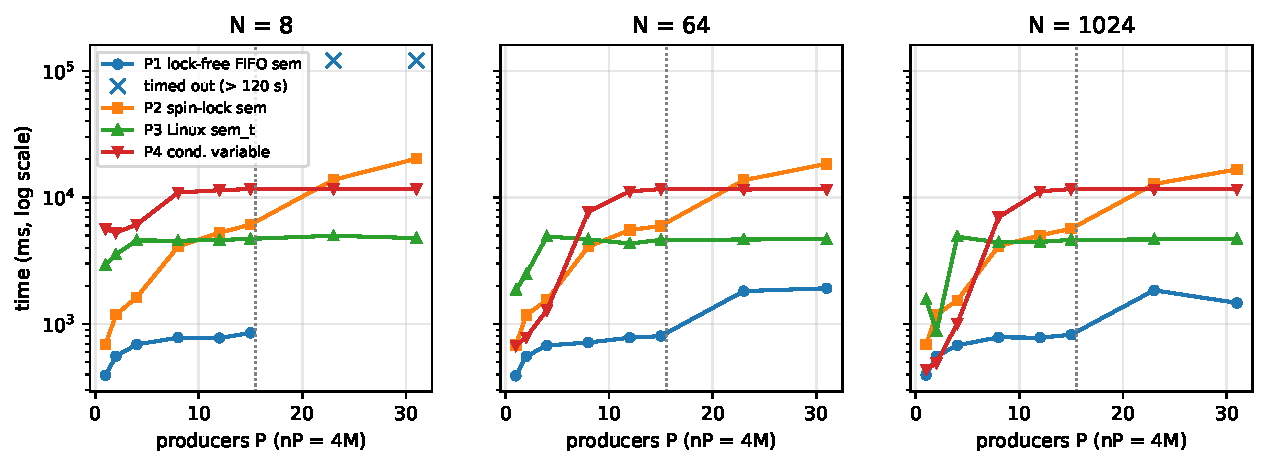
\includegraphics[width=\textwidth]{figs/q1_sweep.pdf}
\caption{Q1: time to pass 4M values from $P$ producers to one consumer (log scale; lower is better). The dotted line marks $P+1 = 16$ threads, the number of hardware threads.
An $\times$ means the run did not finish within 120\,s.}
\label{fig:q1}
\end{figure}

\begin{table}[h]
\centering\small
\begin{tabular}{rlrrrrrrrr}
\toprule
$N$ & Version & $P{=}1$ & $P{=}2$ & $P{=}4$ & $P{=}8$ & $P{=}12$ & $P{=}15$ & $P{=}23$ & $P{=}31$ \\
\midrule
8 & P1 & \textbf{393} & \textbf{557} & \textbf{690} & \textbf{781} & \textbf{775} & \textbf{852} & $>$120k & $>$120k \\
 & P2 & 687 & 1184 & 1623 & 4086 & 5261 & 6106 & 13778 & 20222 \\
 & P3 & 2908 & 3542 & 4577 & 4550 & 4609 & 4709 & \textbf{4982} & \textbf{4769} \\
 & P4 & 5617 & 5272 & 6102 & 10921 & 11409 & 11649 & 11739 & 11671 \\
\midrule
64 & P1 & \textbf{390} & \textbf{556} & \textbf{676} & \textbf{715} & \textbf{779} & \textbf{803} & \textbf{1819} & \textbf{1916} \\
 & P2 & 682 & 1177 & 1548 & 4091 & 5520 & 5966 & 13684 & 18420 \\
 & P3 & 1854 & 2476 & 4915 & 4667 & 4321 & 4619 & 4652 & 4677 \\
 & P4 & 675 & 785 & 1288 & 7713 & 11164 & 11644 & 11561 & 11598 \\
\midrule
1024 & P1 & \textbf{395} & 556 & \textbf{679} & \textbf{785} & \textbf{780} & \textbf{823} & \textbf{1849} & \textbf{1467} \\
 & P2 & 692 & 1184 & 1540 & 4125 & 5020 & 5662 & 12767 & 16658 \\
 & P3 & 1566 & 876 & 4893 & 4412 & 4449 & 4622 & 4659 & 4688 \\
 & P4 & 437 & \textbf{492} & 1005 & 6986 & 11186 & 11646 & 11566 & 11607 \\
\bottomrule
\end{tabular}

\caption{Q1: time in ms for $nP = 4$M values (median of 3; single run for $P \ge 23$). Bold marks the fastest version for each $(N, P)$.}
\label{tab:q1}
\end{table}

\paragraph{P1 with up to 15 producers.}
For every $N$ and every $P \le 15$, P1 was the fastest of the four versions, except at $P = 2$ with $N = 1024$ (discussed under P4 below).
Its time went from 0.39\,s at $P=1$ to 0.80--0.85\,s at $P=15$, i.e.\ about 100--215\,ns per value. At $P=15$ it was 7--7.5$\times$ faster than P2,
5.5--5.8$\times$ faster than P3 and 14--14.5$\times$ faster than P4. We think this comes mainly from three properties of the design:
in the common case \texttt{wait} and \texttt{post} are a single successful CAS each, with no lock to hand over between threads;
waiting threads only read \texttt{grant}, and each \texttt{post} lets exactly one waiter through, so waiters do not compete with each other;
and no thread ever enters the kernel.

\paragraph{P2.}
P2's time grew almost linearly with $P$, from 0.68--0.69\,s at $P=1$ to 5.7--6.1\,s at $P=15$. Our understanding is that all producers that see a positive count
compete for the same lock, and the consumer's \texttt{post} has to win that lock against them before any producer can continue. The test-and-test-and-set lock with
back-off reduced this (Section~1.2) but did not remove it. P2 also slowed down a lot when oversubscribed (13--20\,s at $P = 23, 31$),
which we attribute to lock holders being preempted while the other threads spin.

\paragraph{P3.}
From $P = 4$ on, P3 took 4.3--5.0\,s regardless of $P$ or $N$. We believe that with several producers the semaphore is almost always contended,
so most \texttt{sem\_wait} calls sleep and most \texttt{sem\_post} calls have to wake a sleeper through a system call, which costs on the order of a microsecond per value.
Because sleeping threads do not use the CPU, its time did not change between $P = 15$ and $P = 31$. With a single producer, $N$ made a difference
(2.9\,s at $N=8$ vs 1.6\,s at $N=1024$), presumably because a small buffer fills up immediately and forces the producer to sleep more often.

\paragraph{P4.}
P4 was the slowest version for $P \ge 8$, levelling off at about 11.6\,s. Every \texttt{wait} and \texttt{post} takes the semaphore's mutex, so at this point
up to 15 producers and the consumer queue on one mutex, and a woken waiter has to take the mutex again before it can continue.
With two producers and $N = 1024$, however, P4 was the fastest version (0.49\,s vs 0.56\,s for P1), and with one producer it came close (0.44\,s vs 0.40\,s). In that setting threads rarely have to wait in either version.
One possible explanation, which we have not verified, is that P1's \texttt{FetchAndInc} loads the counter and then does the CAS, which may cost an extra cache-line transfer
when another core wrote the line last, whereas glibc's mutex fast path is a single CAS.

\paragraph{P1 with more threads than hardware threads.}
The result we found most surprising was P1 at $N = 8$ with $P = 23$ and $P = 31$: it did not finish within 120\,s (in an earlier trial a single
$P=23$ run took about 560\,s), while P3 needed under 5\,s. Our explanation is that this follows from combining strict FIFO order with busy-waiting.
With 24 or more threads on 16 hardware threads, some threads are always preempted. A \texttt{post} lets through only the thread holding the next ticket;
if that thread is not running, nobody can use the free slot until the scheduler runs it again, while the other waiters, who may not overtake it, keep spinning.
With $N = 8$ almost all producers are waiting on \texttt{sem\_prod} at any time, so this would happen on almost every value.
With $N = 64$ or $1024$, P1 still finished (1.5--1.9\,s), although more slowly than at $P = 15$. P3 sleeps instead of spinning and was not affected.
We also checked this on fewer CPUs (restricting the program with \texttt{taskset}). With 4 CPUs, P1 was fine with up to 8 producers (0.1--0.3\,s for 1M values),
but with $N = 8$ and $P = 15$ it did not finish 1M values within 60\,s.

As an experiment, we tried a variant of P1 that calls \texttt{sched\_yield()} when a waiter (or the consumer, waiting on a \texttt{full} flag) has spun for a while without progress,
so that a preempted thread can run sooner. FIFO order is unchanged, since the tickets are the same. This removed the problem in our tests (4M values, median of 3: 8.1\,s with 4 CPUs, $N=8$, $P=15$;
3.7\,s and 6.0\,s with 16 CPUs, $N=8$, $P=23$ and $31$) and did not slow down the normal cases (it was even slightly faster: 0.67--0.70\,s vs 0.78--0.80\,s at $N=64$, $P=8, 15$).
However, \texttt{sched\_yield()} gives the CPU to another thread, and the assignment asks that the waiting thread is not context-switched,
so we did not include it in the submitted P1. This means our P1 is best run with $P+1$ at most the number of hardware threads, or with a larger $N$;
with far more threads than cores and a small buffer, it can take minutes.

\paragraph{Effect of $n$.}
\begin{figure}[h]
\centering
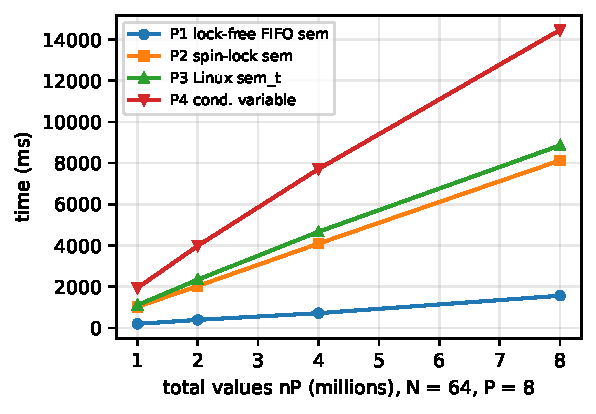
\includegraphics[width=0.45\textwidth]{figs/q1_n.pdf}
\caption{Q1: time vs total number of values ($N = 64$, $P = 8$).}
\label{fig:q1n}
\end{figure}
For every version, the time grew linearly with the number of values (Figure~\ref{fig:q1n}; P1: 0.20, 0.39, 0.72, 1.56\,s for 1, 2, 4, 8M values).
So the cost per value is roughly constant, and we think the 4M values used in the main sweep (at least 0.5\,s per run) are enough to average out measurement noise.
The ranking of the four versions did not depend on $n$.

\paragraph{Testing the FIFO guarantee.}
To check the FIFO property directly, we wrote a separate test program (not included in the submission) that reuses the four semaphores from \texttt{q1\_mpsc.cpp} unchanged.
The semaphore starts at 1, so only one thread passes at a time. $T$ threads each repeat
\emph{take an arrival number (\texttt{FetchAndInc}), \texttt{wait}, log the arrival number, short critical section, \texttt{post}},
for $160{,}000$ passes in total. We count the passes that were \emph{overtaken} (some later arrival passed first), and the worst \emph{bypass}
(the largest number of later arrivals that passed before one thread).

\begin{center}\small
\begin{tabular}{rcccc}
\toprule
$T$ & P1 lock-free FIFO & P2 spin lock & P3 \texttt{sem\_t} & P4 cond.\ var. \\
\midrule
4  & 2 \;(0.001\%), max 2  & 38.4\%, max 81   & 49.7\%, max 941 & 34.6\%, max 779 \\
8  & 1 \;(0.001\%), max 2  & 43.7\%, max 377  & 55.3\%, max 747 & 43.7\%, max 722 \\
15 & 1 \;(0.001\%), max 51 & 60.4\%, max 2491 & 58.3\%, max 848 & 44.8\%, max 424 \\
\bottomrule
\end{tabular}

\smallskip
{\footnotesize Overtaken passes (median of 3 runs) and worst bypass over the 3 runs.}
\end{center}

For P1, at most 5 of the 160{,}000 passes were overtaken in any run. We think these few cases come from the test itself rather than the semaphore:
the arrival number is taken just \emph{before} \texttt{wait} takes its ticket, so a thread that is delayed between the two (for example, by an interrupt) can be overtaken.
This would also explain the single bypass of 51 in one run at $T=15$. The other three semaphores do not promise any order, and in our runs
34--61\% of their passes were overtaken, with single waiters bypassed by hundreds or, in one case, thousands of later arrivals.

\paragraph{Fairness in the producer-consumer program.}
We also wanted to see whether FIFO order makes the producers progress at the same rate. In the real program ($N=64$, $nP=4$M) we recorded when each producer finished,
and report the first producer's finish time as a fraction of the total time (1.0 means all producers finished together; median of 3 runs):

\begin{center}\small
\begin{tabular}{rcccc}
\toprule
$P$ & P1 & P2 & P3 & P4 \\
\midrule
4  & 0.978 & 0.954 & 0.990 & 0.989 \\
8  & 0.999 & 0.879 & 0.970 & 0.995 \\
15 & 0.993 & 0.820 & 0.994 & 0.990 \\
\bottomrule
\end{tabular}
\end{center}

P2 was noticeably unfair, increasingly so with more producers: some producers finished well before others, and in the worst run the first producer was done after only 80\% of the total time.
P1 kept all producers within a few percent of each other. We expected P3 and P4 to be less fair than P1, but over a whole run they were about as fair, even though their individual passes are often out of order.
Our guess is that their reorderings average out over millions of passes, while P2's lock tends to favour the same threads (for example, the thread that has just released the lock may win it again).
So in our measurements, the benefit of FIFO showed up mostly in the waiting time of individual \texttt{wait} calls, and P2 was the only version that was also unfair over a whole run.

\paragraph{Effect of padding the shared variables.}
Late in the project we noticed that \texttt{write\_pointer} and the two semaphores were ordinary neighbouring global variables, so they shared a cache line with each other
and with \texttt{N}, \texttt{n} and \texttt{array}, which every thread reads for every value. We gave each of them its own cache line (Section~1.3) and reran all the experiments
above; all other numbers in this section are from the padded version. To measure the effect itself, we ran the unpadded and the padded build alternately in one session
($N = 8, 64, 1024$; $P = 1, 2$, plus $P = 4, 8, 15$ for $N = 8, 64$; median of 3 each).
P1 became 27--28\% faster at $P=1$ (0.54\,s $\to$ 0.39\,s) and 18--20\% faster at $P=2$ (0.69--0.70\,s $\to$ 0.56\,s), for every $N$.
Our guess is that before, every \texttt{FetchAndInc(\&write\_pointer)} by a producer invalidated the line holding \texttt{N}, which the consumer then had to fetch again.
P2 became 5--29\% faster for $P \ge 2$, which we think is because the two semaphores' locks no longer share a line, so producers spinning on \texttt{sem\_prod}
no longer slow down the consumer's \texttt{sem\_cons}. P3 changed in both directions: with one producer it became 20\% slower at $N = 64$ and $1024$
(1.55\,s $\to$ 1.86\,s and 1.21\,s $\to$ 1.45\,s), but with two producers at $N=64$ it became 33\% faster (2.96\,s $\to$ 1.99\,s). P4 with two producers at $N=1024$
became 17\% slower (0.42\,s $\to$ 0.49\,s). With so few threads every value goes through both semaphores, so perhaps keeping them on one line sometimes meant fewer
cache-line transfers; we do not have a clear explanation for these P3 and P4 cases. All other points we compared changed by less than 10\%, and apart from P1 now also being
fastest at $P=1$, $N=1024$, the ranking of the four versions did not change.


%=====================================================================
\section{Question 2: concurrent graph as an array of linked lists}

\subsection{Data structure and setup}
The graph has $n = 10{,}000$ vertices. \texttt{list[u]} is a \emph{sentinel} node (value $-1$) followed by the sorted list of the out-neighbours of $u$.
The sentinel is never deleted, so every list starts with a node that has a lock, and there is no separate \texttt{head} pointer that could change
between reading it and locking the node it points to.

\textbf{Initial graph.} $m = 500{,}000$ distinct directed edges are drawn from a fixed seed (\texttt{GRAPH\_SEED}), so the initial graph is the same in every run.
The average out-degree is 50 and the density is 0.5\%, far from complete. Each list is laid out in sorted order in one contiguous array of nodes.

\textbf{Operation list.} \texttt{gen\_graph\_ops} writes lines \texttt{op u v} with $u \ne v$ uniform in $[0,n)$.
It fills an array with the exact number of each op type and Fisher--Yates shuffles it, so the three types are \emph{uniformly mixed} over the whole list
(drawing a random type until each quota runs out would leave only the last remaining type at the end of the file).
We used 3 mixes $\times$ 3 sizes (1M, 2M, 4M operations), each with its own file.

\textbf{Work distribution.} As in the class programs, thread $i$ executes the contiguous block $[\,i\cdot\frac{ops}{T}, (i{+}1)\cdot\frac{ops}{T})$ of the op list.
Remainders are handled, so any $T$ works. With $T=1$ every version runs the lock-free sequential code (the class's convention), which gives the sequential baseline.

\textbf{No allocation while timing.} Before the timer starts, each thread gets a \emph{node pool} sized to the number of inserts in its block, with the locks already initialised
(\texttt{pthread\_mutex\_init}, \texttt{pthread\_rwlock\_init} or 0). An insert just takes the next node from its own pool, with no \texttt{malloc} and no shared allocator.
Deleted nodes are not freed during the run. P6 needs this, because a thread walking without locks may still be on a deleted node; we do the same in all versions to keep
them comparable, and all memory is freed after the timer stops.

\subsection{The six versions}
\begin{description}
\item[P1, one mutex for the graph.] Each operation runs the sequential list code inside one global \texttt{pthread\_mutex}.
\item[P2, one mutex per list.] \texttt{list\_lock[u]} protects list $u$. Each lock is padded to a cache line, so locks of different lists do not falsely share.
\item[P3, one mutex per node, hand-over-hand.] The walk holds the lock of \texttt{prev}. To step forward it locks \texttt{curr} and only then releases \texttt{prev}.
  While \texttt{prev} is held, \texttt{curr} cannot be unlinked (that needs \texttt{prev}'s lock) and nothing can be inserted in front of it, so its value can be read safely.
  \emph{Insert and search only need \texttt{prev}} locked at the end of the walk; only delete
  also locks the victim (so that no one is inserting right after it). This saves one lock/unlock pair per insert and search.
\item[P4, one read/write lock per node.] Search walks hand-over-hand with \emph{read} locks only, so concurrent searches share nodes.
  Insert and delete also walk with \emph{read} locks and take a \emph{write} lock only on the node they
  expect to be the final predecessor. A read lock cannot be upgraded to a write lock (two readers trying to upgrade would wait for each other forever),
  so the lock type has to be chosen before locking: they peek at \texttt{node->next} without a lock, which is safe because nodes are never freed during the run.
  This prediction is checked once the lock is held. If it was wrong because the list changed in between (a read-locked node turns out to be the predecessor), the
  operation releases its lock and redoes the walk with write locks on every node, which always succeeds. So almost every operation takes a single write lock.
  Compared with taking write locks all the way down (4M ops, median of 3), this was 6--10\% faster on the 80\% insert mix (at $T=16$: 4.91\,s $\to$ 4.43\,s),
  about 5\% faster on 30/30/40 and about 3\% faster on 10/10/80, which fits with only inserts and deletes benefiting from it.
\item[P5, one cmpxchg spin lock per node.] The same hand-over-hand algorithm as P3, with a cmpxchg spin lock (also used by P6).
  \emph{Optimisation:} as in Question 1, the lock is test-and-test-and-set instead of a CAS in a loop: a waiter spins on an ordinary
  read of the lock word, with the \texttt{pause} instruction, and attempts the CAS only when the lock looks free. Spinning on a read keeps the line in the
  waiter's cache instead of pulling it away from the holder on every iteration. \texttt{pause} also stops a spinning thread from slowing down the other
  hardware thread on the same core. Unlike in Question 1, we did not measure a significant difference from plain test-and-set here (30/30/40, 4M ops, $T=8,16,32$:
  all within run-to-run noise). We think this is because, with 10{,}000 lists, a node's lock is rarely contended, so there is little spinning to save,
  and for the same reason we did not add back-off.
\item[P6, optimistic locking.] Walk with no locks, lock what will be modified, then \emph{validate}
  (\texttt{!prev->deleted \&\& prev->next == curr}, plus \texttt{!curr->deleted} for delete) and retry if validation fails. Delete marks the node
  (\texttt{deleted = 1}) before unlinking it.
  \begin{itemize}
  \item insert, and a delete that does not find the edge, lock only \texttt{prev} (\texttt{prev->next} is the only pointer they rely on);
  \item search takes no locks: it walks and reports the edge only if the node is not marked deleted;
  \item \texttt{CompareAndSet} does not tell the compiler that it orders memory, so the compiler could reuse
        \texttt{prev->next} or \texttt{deleted} loaded \emph{before} the lock, and validation would then pass on stale values. So, as the class code does
        before releasing a lock, we put a compiler barrier (\texttt{asm("":::"memory")}) after acquiring and before releasing.
        We also use volatile loads for the lock-free walk, and put a barrier before publishing a new node, so its fields are written before \texttt{prev->next} points to it
        (x86 keeps stores in order, so no hardware fence is needed).
  \end{itemize}
\end{description}

\subsection{Optimisations (summary)}
\begin{itemize}
\item \textbf{Sentinel head per list:} every list starts with a lockable node, with no head pointer to protect.
\item \textbf{Fewer locks per operation (P3, P5, P6):} insert holds only \texttt{prev} instead of \texttt{prev} and \texttt{curr}, and in P3/P5 the walk holds one lock instead of two; only delete also locks the victim.
\item \textbf{Read-lock walk for writers (P4):} insert/delete take a single write lock, on the last predecessor; 3--10\% faster.
\item \textbf{Lock-free search (P6).}
\item \textbf{Test-and-test-and-set spin lock (P5, P6).}
\item \textbf{Per-thread node pools:} no \texttt{malloc} or lock initialisation while timing, and no shared allocator.
\item \textbf{Initial lists laid out contiguously in sorted order}, for better locality.
\item \textbf{Cache-line padding} of everything that threads write during the run and that would otherwise share a line: per-list locks (P2), list heads (whose locks every operation on that list takes in P3--P6), P1's global lock, the per-thread pool counters and the per-thread result counters.
  We added the last three paddings after the main sweep; rerunning both mixes at 2M ops with 1--32 threads (3 runs each), we saw no difference beyond run-to-run noise, so the tables below are from the earlier build.
\item \textbf{Uniformly shuffled operation list} and work split that handles any thread count.
\end{itemize}

\subsection{Results}
\textbf{Experiments.} For each of the three operation mixes and three operation counts (1M, 2M, 4M) we ran all six versions with
$T \in \{1, 2, 4, 8, 12, 16, 24, 32\}$ threads, 3 times each, and report the median: 1{,}296 runs in total, all of which passed the correctness check.
$T \le 16$ fits in the 8 cores / 16 hardware threads, and $T = 24, 32$ oversubscribe the machine. With $T=1$ every version runs the same sequential code,
so differences at $T=1$ come only from the node layout (P3 and P4 nodes carry a 40-byte mutex or a 56-byte rwlock).
One sequential run (P5, 80/10/10, 4M) took 909\,s because the laptop went to sleep during it; taking the median of 3 keeps it out of all reported numbers.

\textbf{Choice of 1M--4M operations.} The initial graph is fixed, but the operations change it. Because $u, v$ are random and the graph is sparse,
almost every insert succeeds and almost every delete misses, so the graph grows by roughly the insert fraction times the number of operations.
With 80\% inserts, 4M operations grow it from 0.5M to about 3.7M edges (average list length 50 $\to$ 370), and the time per operation grows with it
(the sequential time was 1.3\,s for 1M, 5.6\,s for 2M and 29\,s for 4M operations). At 4M operations the nodes no longer fit in the 16\,MB L3 cache,
so we expect most steps along a list to miss in the cache. We first planned 2M/4M/8M, but estimated that the full sweep would take more than 10 hours, so we used 1M/2M/4M.
Even the fastest configurations at 4M operations take about 0.1\,s.

\begin{figure}[p]
\centering
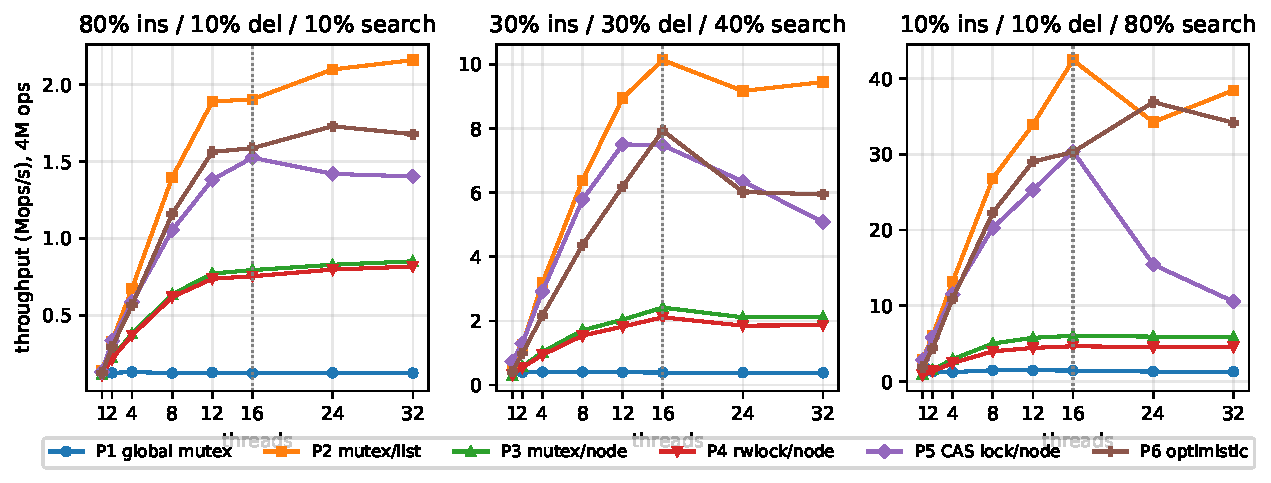
\includegraphics[width=\textwidth]{figs/q2_tput_4M.pdf}\\[1.2em]
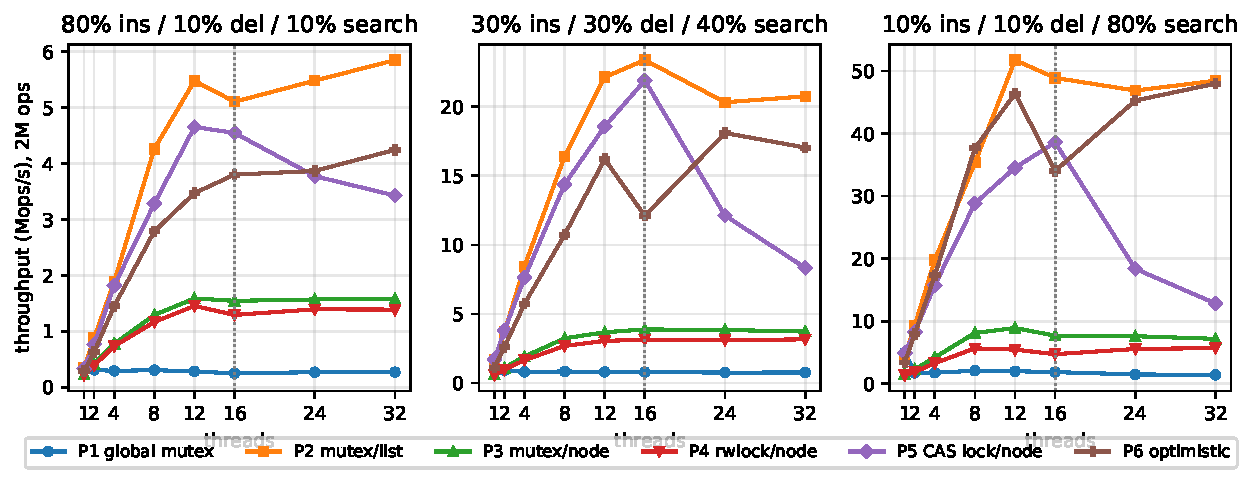
\includegraphics[width=\textwidth]{figs/q2_tput_2M.pdf}\\[1.2em]
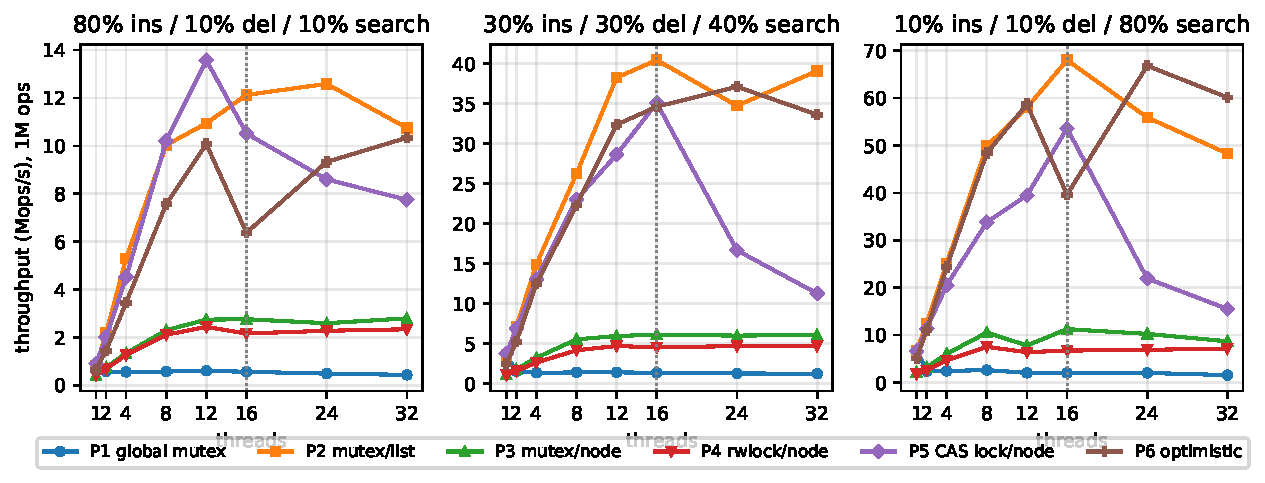
\includegraphics[width=\textwidth]{figs/q2_tput_1M.pdf}
\caption{Q2: throughput (millions of operations per second; higher is better) vs threads for 4M (top), 2M and 1M (bottom) operations.
The dotted line marks 16 hardware threads.}
\label{fig:q2}
\end{figure}

\begin{table}[h]
\centering\footnotesize
\begin{tabular}{llrrrrrrrr}
\toprule
Mix & Ops & $T{=}1$ & $T{=}2$ & $T{=}4$ & $T{=}8$ & $T{=}12$ & $T{=}16$ & $T{=}24$ & $T{=}32$ \\
\midrule
80/10/10 & 1M & P5 (0.9) & P2 (2.2) & P2 (5.3) & P5 (10.2) & P5 (13.6) & P2 (12.1) & P2 (12.6) & P2 (10.7) \\
80/10/10 & 2M & P1 (0.4) & P2 (0.9) & P2 (1.9) & P2 (4.3) & P2 (5.5) & P2 (5.1) & P2 (5.5) & P2 (5.8) \\
80/10/10 & 4M & P2 (0.1) & P5 (0.3) & P2 (0.7) & P2 (1.4) & P2 (1.9) & P2 (1.9) & P2 (2.1) & P2 (2.2) \\
\midrule
30/30/40 & 1M & P5 (3.7) & P2 (7.1) & P2 (14.9) & P2 (26.2) & P2 (38.2) & P2 (40.4) & P6 (37.1) & P2 (39.1) \\
30/30/40 & 2M & P5 (1.7) & P5 (3.8) & P2 (8.5) & P2 (16.4) & P2 (22.1) & P2 (23.4) & P2 (20.3) & P2 (20.7) \\
30/30/40 & 4M & P5 (0.7) & P5 (1.3) & P2 (3.2) & P2 (6.4) & P2 (8.9) & P2 (10.1) & P2 (9.2) & P2 (9.4) \\
\midrule
10/10/80 & 1M & P1 (6.9) & P2 (12.4) & P2 (25.1) & P2 (49.9) & P6 (58.7) & P2 (68.0) & P6 (66.8) & P6 (60.1) \\
10/10/80 & 2M & P1 (5.0) & P2 (9.3) & P2 (19.8) & P6 (37.6) & P2 (51.7) & P2 (48.9) & P2 (46.9) & P2 (48.4) \\
10/10/80 & 4M & P2 (2.9) & P2 (6.0) & P2 (13.2) & P2 (26.8) & P2 (33.9) & P2 (42.4) & P6 (36.9) & P2 (38.4) \\
\bottomrule
\end{tabular}

\caption{Q2: fastest version for every configuration, with its throughput in Mops/s. All times are in Appendix~\ref{app:q2}.}
\label{tab:q2best}
\end{table}

\paragraph{Overview.}
Figure~\ref{fig:q2} and Table~\ref{tab:q2best} show a similar picture for every mix and size. The one-mutex-per-list version (P2) was the fastest or close to it in almost all configurations.
The optimistic version (P6) and the hand-over-hand spin-lock version (P5) came next, the hand-over-hand pthread versions (P3, P4) were 2--7$\times$ slower than P2,
and the global lock (P1) did not scale. For P2 with 16 threads and 4M operations, the speed-up over the sequential run was
about 12--14$\times$ (80/10/10), 13--17$\times$ (30/30/40) and 14--15$\times$ (10/10/80). We give ranges because the sequential time varied a lot between runs:
P1, P2 and P5 run identical sequential code at $T=1$, and their nine runs for 30/30/40 with 4M operations took between 5.2 and 7.3\,s
(the lower end of each range uses the fastest of these nine runs, the upper end their median). These speed-ups are higher than the 8 physical cores. Our interpretation is that the work is dominated by
cache misses while following list pointers, and the two hardware threads of a core can overlap their misses.
Already at 2--8 threads the speed-up was slightly above the number of threads (e.g.\ 2.1--2.4$\times$ at $T=2$). We think this is at least partly because the sequential runs
were often slow: when we repeated the 30/30/40, 4M sequential run seven times, it took between 4.8 and 9.0\,s, while 2-thread runs stayed at 2.9--3.0\,s.
Our laptop was in a power-saving profile, and we suspect a single busy thread is not clocked or scheduled consistently, but we did not investigate this further.

\paragraph{P1 (one global mutex).}
P1 was slower with 2 threads than with 1 in every configuration (e.g.\ 1.4\,s $\to$ 3.0\,s for 10/10/80, 4M), and stayed flat or got slower with more threads.
This is what we expected, since only one operation can run at a time. We think the slow-down comes from the mutex and the list data moving between cores,
and from waiting threads being put to sleep and woken up by the contended mutex.

\paragraph{P2 (one mutex per list).}
With 10{,}000 lists and uniformly random $u$, two threads should rarely work on the same list at the same time, so we expect the per-list mutexes to be almost uncontended.
Each operation then costs one lock/unlock pair plus the sequential traversal, nothing is written while walking the list, and the nodes stay at 16 bytes.
P2's time dropped at least in proportion to the number of threads up to 8 threads (see the note on the sequential time above), improved a little more up to 16 (hyper-threading),
and stayed about the same at 24--32 threads.

\paragraph{P3 and P4 (pthread lock per node).}
At 16 threads and 4M operations, P3 was 2.4$\times$ (80/10/10), 4.2$\times$ (30/30/40) and 7.1$\times$ (10/10/80) slower than P2, and P4 was slower than P3. We see two likely reasons:
\begin{itemize}
\item every node visited needs a lock and an unlock, and both write to the node, so walking a list turns into a series of writes;
      nodes near the start of each list, especially the sentinel that every operation on that list locks, then have to move between cores;
\item the nodes are bigger (56 bytes with a mutex, 72 with an rwlock, vs 16), so each list covers 3.5--4.5$\times$ more cache lines.
      We could see this even at $T = 1$, where P3/P4 run the same sequential code as P1/P2 but took 2--3$\times$ longer on the 10/10/80 and 30/30/40 mixes
      (e.g.\ 4.2\,s and 4.7\,s vs 1.4\,s for 10/10/80, 4M).
\end{itemize}
The gap to P2 was smallest for the 80\% insert mix, which we think is because there the graph grows the most and all versions spend most of their time on cache misses.

We expected the read/write locks of P4 to help with the 80\% search mix, since searches can share nodes. This did not happen: P4 was 5--30\% slower than P3 in every mix.
Our understanding is that taking a read lock still writes to the lock word (to update the reader count), so it moves the cache line just like a mutex, and that glibc's rwlock is more expensive than its mutex.
Sharing would only help when readers actually wait for each other, which we expect to be rare with 10{,}000 lists.
The read-locked walk for insert/delete (Section~2.2) made P4 3--10\% faster, but it was still behind P3.

\paragraph{P5 (spin lock per node).}
P5 uses the same hand-over-hand algorithm as P3, but with a 4-byte spin lock, so its nodes are as small as P1/P2's and taking an uncontended lock is cheaper than \texttt{pthread\_mutex\_lock}.
Up to 12--16 threads it was 2--5$\times$ faster than P3 and within 10--40\% of P2, and it was even the fastest version for 80/10/10 with 1M operations at 8 and 12 threads.
Above 16 threads its throughput dropped sharply: for 10/10/80 with 4M operations, from 30 to 11\,Mops/s between $T=16$ and $T=32$.
We think this is the same effect as for P1 in Question 1. When the OS preempts a thread that holds a node lock, the threads that reach that node spin until the holder runs again,
and because every operation on a list passes through the first few nodes, one preempted holder can block several threads.

\paragraph{P6 (optimistic locking).}
P6 walks without locks, locks one or two nodes only for a short time at the end, and does not lock at all for searches. Up to 16 threads it was 20--40\% behind P2.
We think this is because it does the same traversal plus validation and occasional retries, with a slightly larger node (24 bytes, for the \texttt{deleted} flag),
while P2's locks are rarely contended in this setting anyway. Unlike P5, P6 did not slow down sharply above 16 threads; in most configurations it was about as fast at 24--32 threads as at 16.
Our explanation is that it holds its locks for such a short time that a preempted thread rarely blocks others.
For the search-heavy mix this brought it close to P2 at 24--32 threads (within about 10\%, and sometimes faster: 10/10/80, 4M, $T=24$: 0.11\,s vs 0.12\,s;
10/10/80, 1M, $T=32$: 17\,ms vs 21\,ms). For the other two mixes it stayed clearly behind P2 at 2M and 4M operations (13--59\% slower at $T=24, 32$).

\paragraph{Effect of the operation mix.}
The search-heavy mix (10/10/80) ran fastest, as the graph barely grows (+0.4M edges at 4M operations) and searches do not modify anything.
The insert-heavy mix (80/10/10) was by far the slowest, as the graph grows to more than 7$\times$ its initial size.
The mix also changed the gaps between versions: with more searches, the cost of locking every node (P3, P4) mattered more relative to the traversal, and P6's lock-free searches helped more.

\paragraph{Effect of the number of operations.}
More operations always gave lower throughput, because the lists get longer (strongly for 80/10/10, only slightly for 10/10/80). The ranking of the versions was the same for 1M, 2M and 4M operations.
Some 1M configurations finish in 15--100\,ms, so those numbers are noisier. When we repeated some 4M runs at a different time,
the results varied by up to 35\% at $T=16$ on our laptop, so we only draw conclusions from differences that are larger than this and consistent across all three sizes.

\paragraph{Summary.}
In our setup (many vertices and uniformly random operations), contention on any single list was low, and the simplest fine-grained scheme, one lock per list (P2), performed best.
Locking every node added lock operations and larger nodes without much benefit here. Among the per-node schemes, optimistic locking (P6) performed best and was the least affected by oversubscription.
We would expect the per-node schemes to do relatively better on a graph with few vertices and long, frequently accessed lists, but we did not test this.


\appendix
\section{All Question 2 timings}
\label{app:q2}
Median of 3 runs, in ms. Bold marks the fastest version for each operation count and thread count.

\begin{center}\scriptsize
\begin{tabular}{llrrrrrrrr}
\toprule
\multicolumn{10}{c}{\textbf{80\% ins / 10\% del / 10\% search} (time in ms)} \\
\midrule
Ops & Ver. & $T{=}1$ & $T{=}2$ & $T{=}4$ & $T{=}8$ & $T{=}12$ & $T{=}16$ & $T{=}24$ & $T{=}32$ \\
\midrule
1M & P1 & 1255 & 1726 & 1778 & 1735 & 1643 & 1763 & 2035 & 2282 \\
 & P2 & 1247 & \textbf{459} & \textbf{189} & 100 & 91 & \textbf{82} & \textbf{79} & \textbf{93} \\
 & P3 & 2301 & 1331 & 746 & 434 & 364 & 362 & 385 & 357 \\
 & P4 & 2329 & 1437 & 787 & 472 & 410 & 462 & 439 & 427 \\
 & P5 & \textbf{1092} & 496 & 221 & \textbf{98} & \textbf{74} & 95 & 116 & 129 \\
 & P6 & 1541 & 690 & 290 & 132 & 99 & 157 & 107 & 97 \\
\midrule
2M & P1 & \textbf{5603} & 6431 & 6827 & 6519 & 7061 & 8049 & 7403 & 7400 \\
 & P2 & 5762 & \textbf{2269} & \textbf{1060} & \textbf{469} & \textbf{365} & \textbf{392} & \textbf{365} & \textbf{342} \\
 & P3 & 8820 & 4802 & 2578 & 1547 & 1259 & 1294 & 1274 & 1267 \\
 & P4 & 9168 & 5112 & 2719 & 1713 & 1375 & 1545 & 1435 & 1440 \\
 & P5 & 5970 & 2606 & 1099 & 609 & 430 & 440 & 530 & 583 \\
 & P6 & 6878 & 3163 & 1380 & 717 & 576 & 526 & 517 & 471 \\
\midrule
4M & P1 & 29090 & 31989 & 30696 & 32461 & 31501 & 32341 & 32073 & 32319 \\
 & P2 & \textbf{28615} & 12170 & \textbf{5923} & \textbf{2865} & \textbf{2117} & \textbf{2100} & \textbf{1906} & \textbf{1852} \\
 & P3 & 34859 & 17890 & 10541 & 6296 & 5187 & 5040 & 4830 & 4702 \\
 & P4 & 36199 & 18371 & 10819 & 6476 & 5427 & 5308 & 5019 & 4896 \\
 & P5 & 30261 & \textbf{11950} & 6830 & 3800 & 2895 & 2623 & 2818 & 2851 \\
 & P6 & 32270 & 13653 & 7068 & 3449 & 2560 & 2520 & 2313 & 2384 \\
\bottomrule
\end{tabular}
\vspace{1em}

\begin{tabular}{llrrrrrrrr}
\toprule
\multicolumn{10}{c}{\textbf{30\% ins / 30\% del / 40\% search} (time in ms)} \\
\midrule
Ops & Ver. & $T{=}1$ & $T{=}2$ & $T{=}4$ & $T{=}8$ & $T{=}12$ & $T{=}16$ & $T{=}24$ & $T{=}32$ \\
\midrule
1M & P1 & 280 & 650 & 734 & 713 & 706 & 741 & 784 & 805 \\
 & P2 & 278 & \textbf{141} & \textbf{67} & \textbf{38} & \textbf{26} & \textbf{25} & 29 & \textbf{26} \\
 & P3 & 863 & 554 & 309 & 181 & 168 & 163 & 167 & 164 \\
 & P4 & 932 & 633 & 378 & 239 & 213 & 220 & 213 & 212 \\
 & P5 & \textbf{268} & 145 & 77 & 43 & 35 & 29 & 60 & 89 \\
 & P6 & 407 & 190 & 80 & 45 & 31 & 29 & \textbf{27} & 30 \\
\midrule
2M & P1 & 1257 & 2168 & 2460 & 2366 & 2463 & 2494 & 2613 & 2601 \\
 & P2 & 1197 & 541 & \textbf{237} & \textbf{122} & \textbf{90} & \textbf{86} & \textbf{98} & \textbf{96} \\
 & P3 & 3174 & 1803 & 1039 & 617 & 544 & 515 & 520 & 536 \\
 & P4 & 3422 & 2037 & 1202 & 743 & 653 & 638 & 643 & 631 \\
 & P5 & \textbf{1158} & \textbf{528} & 262 & 139 & 108 & 91 & 165 & 240 \\
 & P6 & 1795 & 766 & 348 & 186 & 124 & 165 & 111 & 117 \\
\midrule
4M & P1 & 6679 & 10008 & 9758 & 9791 & 9998 & 10203 & 10354 & 10435 \\
 & P2 & 6880 & 3207 & \textbf{1256} & \textbf{627} & \textbf{447} & \textbf{395} & \textbf{436} & \textbf{424} \\
 & P3 & 12760 & 6938 & 3894 & 2343 & 1962 & 1655 & 1894 & 1879 \\
 & P4 & 12713 & 7309 & 4245 & 2593 & 2192 & 1893 & 2157 & 2142 \\
 & P5 & \textbf{5457} & \textbf{3081} & 1372 & 693 & 533 & 535 & 630 & 787 \\
 & P6 & 9579 & 4057 & 1848 & 917 & 646 & 504 & 665 & 673 \\
\bottomrule
\end{tabular}
\vspace{1em}

\begin{tabular}{llrrrrrrrr}
\toprule
\multicolumn{10}{c}{\textbf{10\% ins / 10\% del / 80\% search} (time in ms)} \\
\midrule
Ops & Ver. & $T{=}1$ & $T{=}2$ & $T{=}4$ & $T{=}8$ & $T{=}12$ & $T{=}16$ & $T{=}24$ & $T{=}32$ \\
\midrule
1M & P1 & \textbf{145} & 421 & 410 & 379 & 489 & 490 & 493 & 633 \\
 & P2 & 150 & \textbf{80} & \textbf{40} & \textbf{20} & 17 & \textbf{15} & 18 & 21 \\
 & P3 & 451 & 314 & 165 & 95 & 128 & 89 & 97 & 115 \\
 & P4 & 540 & 389 & 213 & 133 & 156 & 148 & 145 & 139 \\
 & P5 & 150 & 88 & 49 & 30 & 25 & 19 & 46 & 64 \\
 & P6 & 197 & 90 & 41 & 21 & \textbf{17} & 25 & \textbf{15} & \textbf{17} \\
\midrule
2M & P1 & \textbf{401} & 1151 & 1130 & 960 & 995 & 1072 & 1339 & 1411 \\
 & P2 & 475 & \textbf{215} & \textbf{101} & 57 & \textbf{39} & \textbf{41} & \textbf{43} & \textbf{41} \\
 & P3 & 1273 & 868 & 476 & 246 & 224 & 260 & 263 & 278 \\
 & P4 & 1438 & 1055 & 607 & 353 & 366 & 423 & 359 & 350 \\
 & P5 & 407 & 241 & 127 & 69 & 58 & 52 & 109 & 156 \\
 & P6 & 586 & 251 & 115 & \textbf{53} & 43 & 59 & 44 & 42 \\
\midrule
4M & P1 & 1414 & 3016 & 3233 & 2699 & 2724 & 2756 & 3071 & 3102 \\
 & P2 & \textbf{1374} & \textbf{665} & \textbf{303} & \textbf{149} & \textbf{118} & \textbf{94} & 117 & \textbf{104} \\
 & P3 & 4174 & 2577 & 1363 & 798 & 694 & 663 & 675 & 684 \\
 & P4 & 4729 & 2924 & 1647 & 1005 & 902 & 860 & 881 & 877 \\
 & P5 & 1409 & 690 & 348 & 197 & 158 & 132 & 259 & 379 \\
 & P6 & 2116 & 916 & 366 & 179 & 138 & 132 & \textbf{108} & 117 \\
\bottomrule
\end{tabular}
\vspace{1em}


\end{center}

\end{document}
